%%%%%%%%%%%%%%%%%%%%% chapter.tex %%%%%%%%%%%%%%%%%%%%%%%%%%%%%%%%%
%
% sample chapter
%
% Use this file as a template for your own input.
%
%%%%%%%%%%%%%%%%%%%%%%%% Springer-Verlag %%%%%%%%%%%%%%%%%%%%%%%%%%

%\motto{Use the template \emph{chapter.tex} to style the various elements of your chapter content.}
\chapter{An Overview of LTE Advanced}
\label{overview-lte} % Always give a unique label
% use \chaptermark{}
% to alter or adjust the chapter heading in the running head

%\abstract*{Each chapter should be preceded by an abstract (10--15 lines long) that summarizes the content. The abstract will appear \textit{online} at \url{www.SpringerLink.com} and be available with unrestricted access. This allows unregistered users to read the abstract as a teaser for the complete chapter. As a general rule the abstracts will not appear in the printed version of your book unless it is the style of your particular book or that of the series to which your book belongs.
%Please use the 'starred' version of the new Springer \texttt{abstract} command for typesetting the text of the online abstracts (cf. source file of this chapter template \texttt{abstract}) and include them with the source files of your manuscript. Use the plain \texttt{abstract} command if the abstract is also to appear in the printed version of the book.}

\abstract{This chapter provides a high-level overview of LTE-Advanced (LTE-A) networks and associated technologies to form a basis for discussion of the co-existence issues that exist for unlicensed LTE and Wi-Fi. Understanding the underlying architecture and protocols employed in LTE-A networks will provide readers a comparative framework to grasp how, and at what levels, LTE and Wi-Fi networks may interact and interfere with each other, and form a greater understanding of the challenges to be address in designing coexistence mechanisms. Specifically, this chapter will overview the LTE-A network, its capabilities and protocols, with specific emphasis on the physical layer and medium access sub-layers to illuminate specific sources of co-existence issues. Proposed changes which may be included in future LTE releases are discussed in the context of LTE/Wi-Fi coexistence.}


\section{System Overview}
\label{sys-overview}%TODO: How much of these acroyms should be spelled out?  Should the reader just refer to the acronym list at the beginning of the book?
The enhancements to the Long Term Evolution/System Architecture Evolution (LTE-SAE) to meet the requirements set out for fourth generation (4G) cellular networks are collectively known as LTE-Advanced, and were formalized in 3GPP TR 36.913, releases 10 through 13 \cite{tr36913}.  LTE itself was a logical evolution from the GSM/EDGE and UMTS/GPRS/HSPA technologies used in previous generations to meet the increasing demands for higher data rates and improved quality of service. LTE meets these demands at the access level through improved spectral efficiency, using OFMDA and SC-FDMA for downlink and uplink, respectively, and improved mobility support and cell edge data rates through enhanced adaptive modulation and bandwidth selection and downlink spatial multiplexing support. To support these gains beyond the access layer, LTE transitioned to an all IP packet switched core network with the introduction of the evolved packet core, and a flattened network architecture of enhanced base stations called evolved NodeB's (eNB) which are interconnected via high-speed.  Combined, this allowed LTE networks to significantly increase user data rates and reduce control and user plane latency and connection set-up and handover times.  

\subsection{Network Architecture}
\label{net-arch}
The requirements to provide high data rates while supporting high-speed mobility requires the ability to set up and tear down user connections and manage inter-cell handoffs with as little latency as possible.  The hierarchical structure consisting of base stations or NodeBs connected to a central controller which had been used in past cellular networks requires additional hops in both data transmissions and hand off negotiation which can introduce significant delay as the controller manages handoffs betweens several pairs of base stations, as well as all other voice and data traffic.  For many increasingly ubiquitous end-user applications, such as online gaming and video conferencing, the additional latency in connection set up and handover can impair the user quality of experience.  

%TODO: expand from content of reference tr36300
To meet these requirements, LTE adopted the flat architecture shown in Fig. \ref{figs:LTE-A-Network} and migrated the functions of radio network, medium access control, handoff request, negotiation, and managements, as well as some other truly local functions, to the eNBs themselves and provided high-speed, low latency, connections between the eNBs in a mesh configuration \cite{tr36300}. 
%TODO:better figure?
\begin{figure}[!ht]
	\centering
	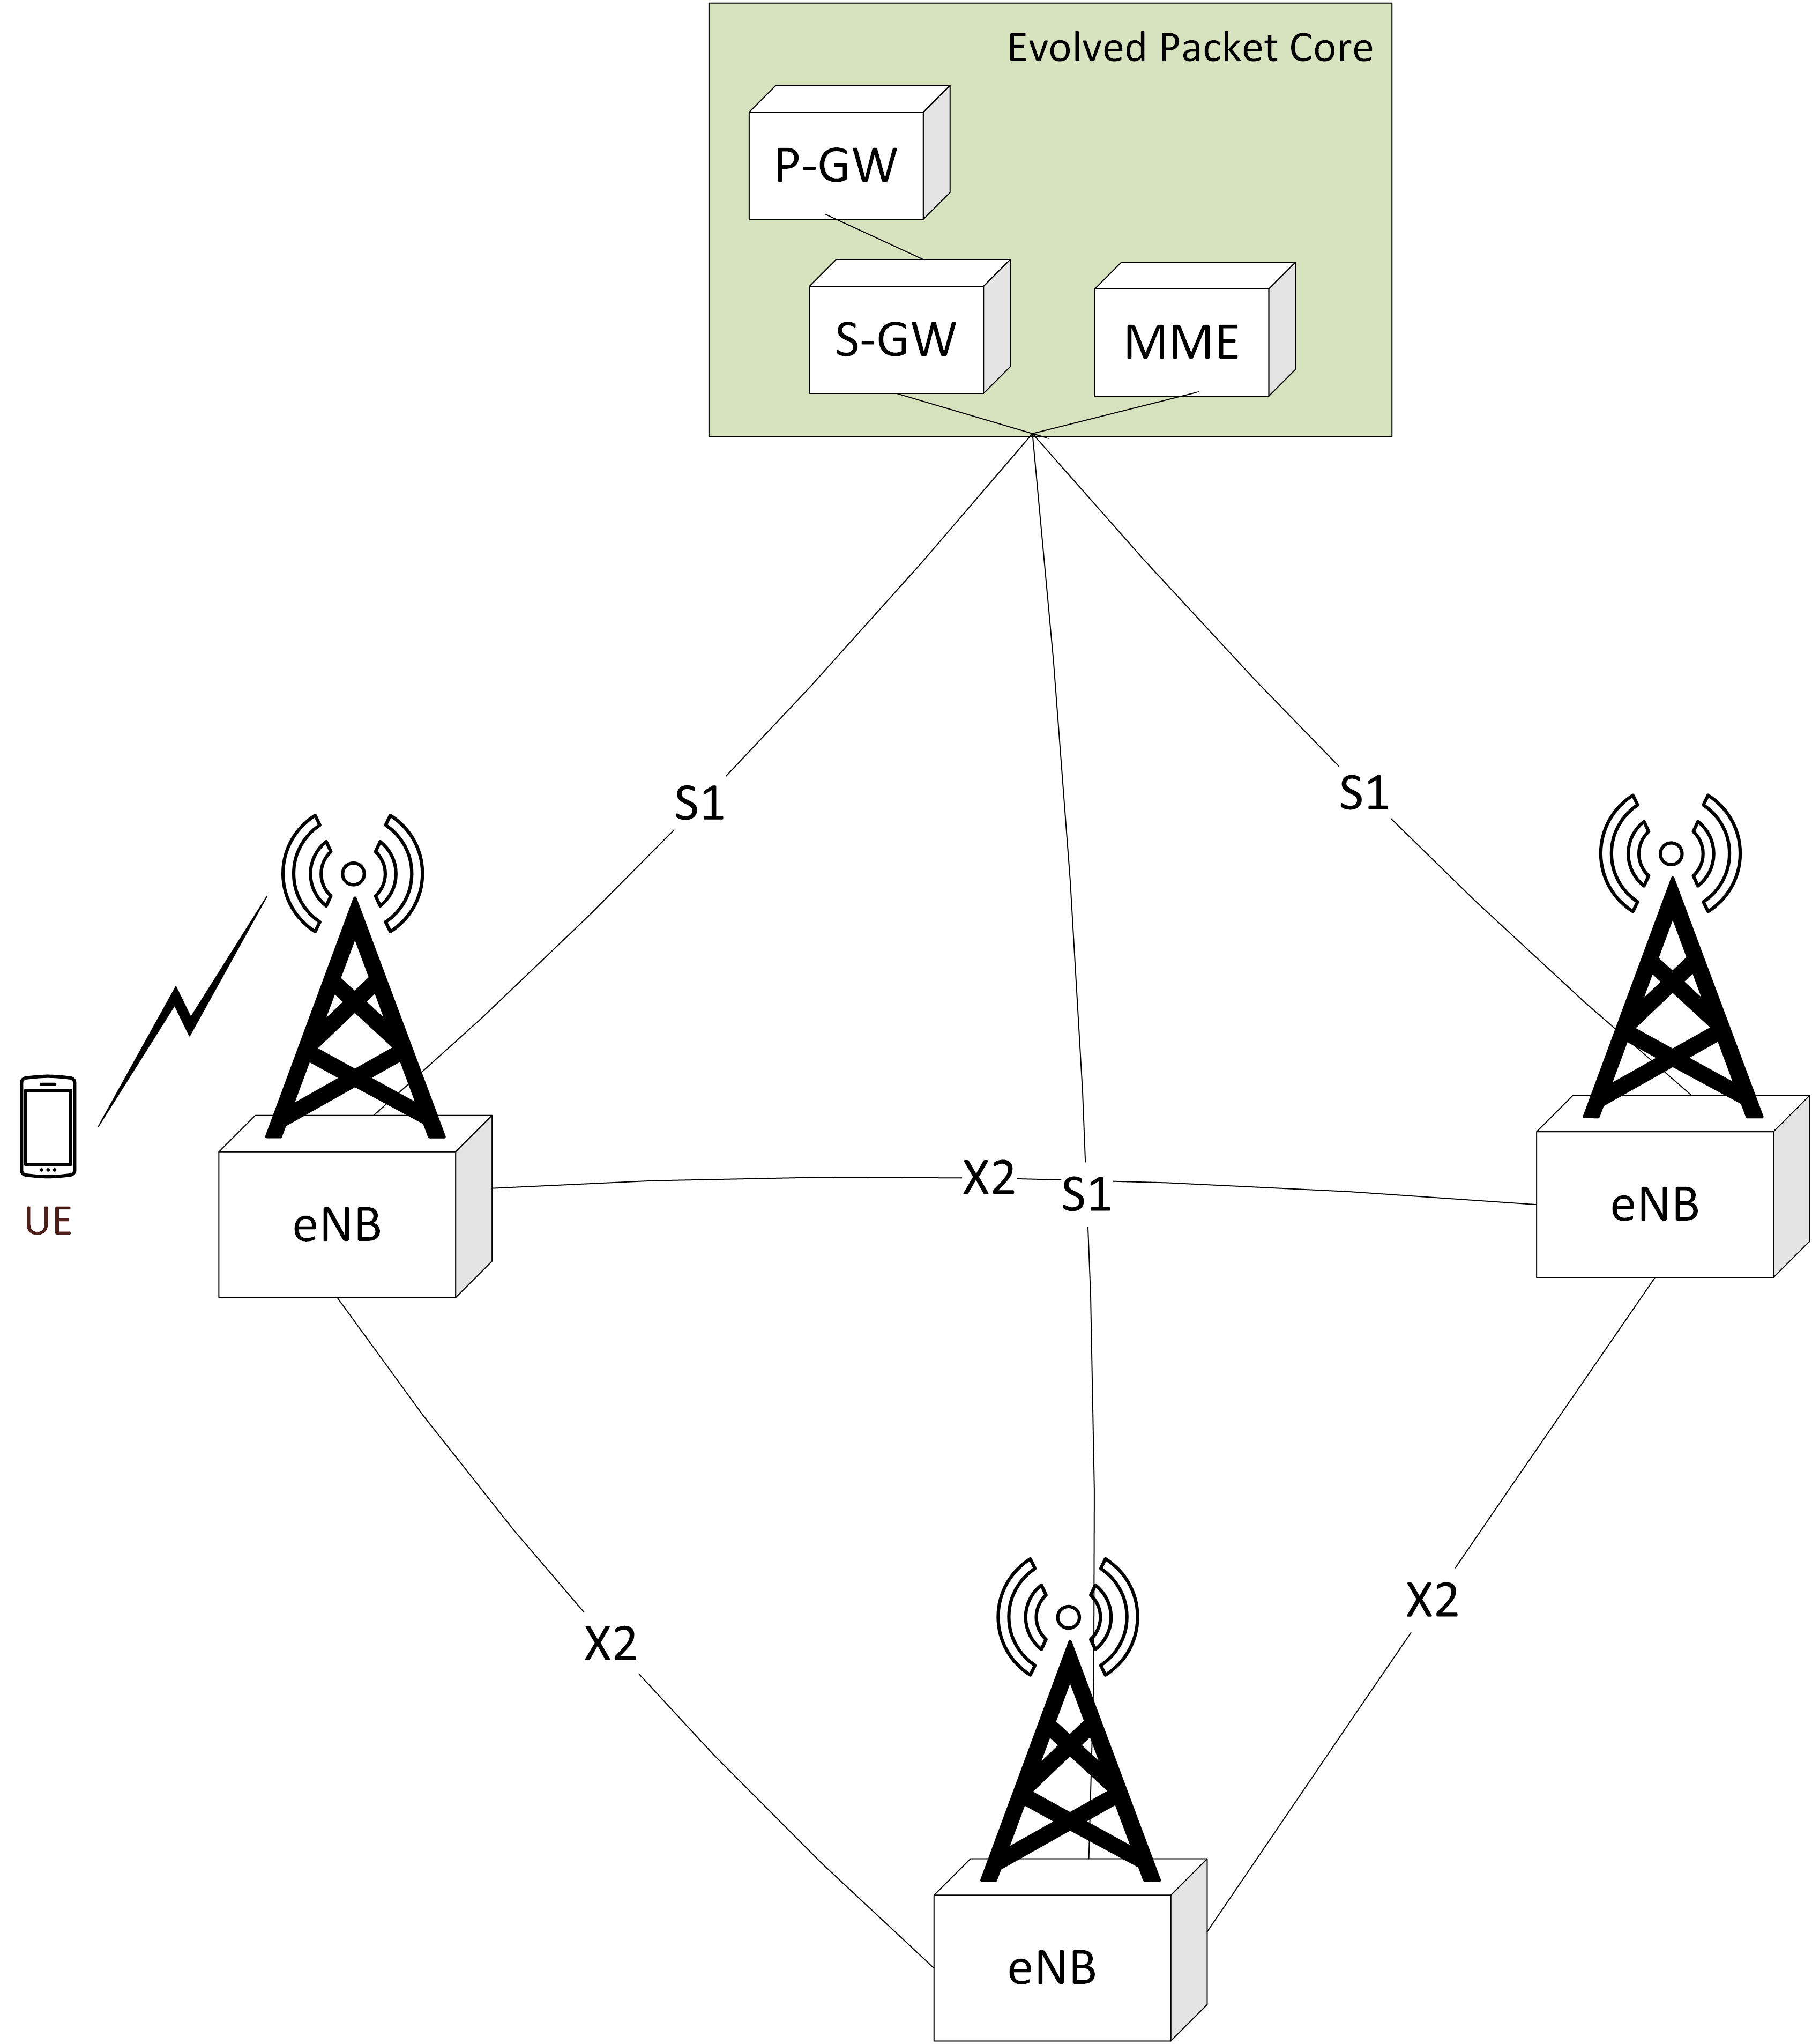
\includegraphics[width=2.5in]{figures3/lteAnet}
	\caption{Basic structure of LTE-A cellular network.}
	\label{figs:LTE-A-Network}
\end{figure}
The global functions and connections to external networks are handled at the evolved packet core (EPC in the the figure). The mobile management entity (MME) handles authentication, authorization and accounting functions, among others.  The packet data network gateway (P-GW) and serving gateway (S-GW) handle user data packet forwarding, filtering, and usage tracking, as well as acting as a mobility anchor for inter-eNB and inter-RAT handovers.  The functional split between the various components of the network is shown in further detail in Fig. \ref{figs:funcSplit}.

%TODO: Figure MUST be changed as it is taken from 3GPP doc for reference/placeholder only
\begin{figure}[!ht]
	\centering
	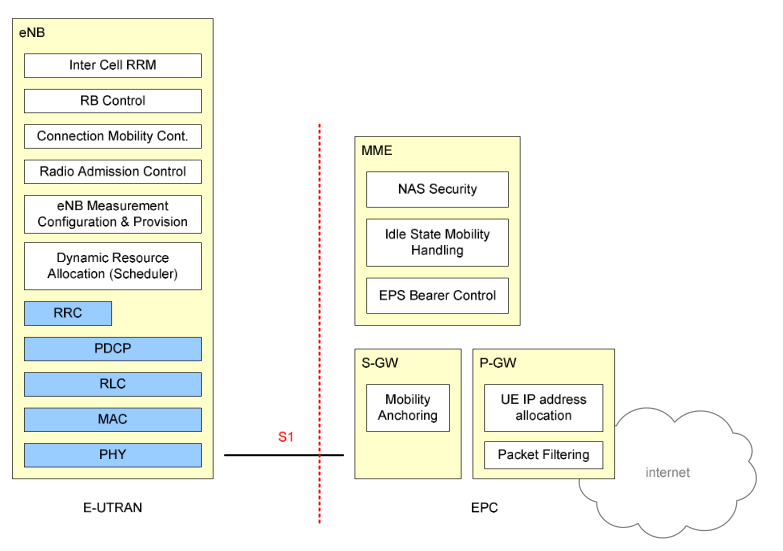
\includegraphics[width=4.25in]{figures3/functionalsplit}
	\caption{Functional split between eNodeB and evolved packet core.}
	\label{figs:funcSplit}
\end{figure}

The distributed radio network and medium access control allows eNBs to quickly adapt to changing radio medium condition and user scheduling based on local information.  The low-latency X2 interface connections between eNBs allows for fast user handover, including forwarding of queued data for seamless user experience.  Additionally, with direct connections between neighbouring cells, this architecture facilitates more effective multi-point transmission and reception coordination and inter-cell interference and load management, independent of conditions in other areas of the network.  

\subsection{Capabilities and Features}

While the gains made by LTE were significant, they fell short of the requirements set out for 4G networks by the International Telecommunications Union, specifically in the case of peak data rates, spectral efficiency, and cell edge performance \cite{itu-advanced}. Some important ITU requirements and achieved performance levels for LTE and LTE-A are highlighted in Table \ref{perf-table}PLACEHOLDER:

%TODO: verify the contents/details of this table and expand if possibe
\begin{table}
	\caption{ITU-A Requirements for 4G vs. LTE/LTE-A Achievements \cite{lte-3gpp}\cite{lteA-3gpp}\cite{itu-advanced}\cite{abdullah}}
	\label{perf-table}      
	\begin{tabular}{p{4.8cm}p{2.4cm}p{2.4cm}p{2.4cm}}
		\hline\noalign{\smallskip}
		Description/Requirements & ITU-A & LTE & LTE-A   \\
		\noalign{\smallskip}\svhline\noalign{\smallskip}
		DL peak spectral efficiency (bps/Hz) &  15   & 15  & 30 \\
		UL peak spectral efficiency (bps/Hz)& 6.75  & 3.75  & 15 \\
		Min. cell edge spectral \\ \hspace{0.8em} efficiency (bps/Hz) & 0.04 & 0.024 & 0.04 \\
		DL Peak data rates (Mbps) & 1000$^1$  & 300 & 1000 \\
		UL Peak data rates (Mbps) & 1000$^1$  & 75 & 500 \\
		Scalable bandwidth up to (MHz) & 40 & 20  & 100$^2$ \\
		
		\noalign{\smallskip}\hline\noalign{\smallskip}
	\end{tabular}
	$^1$ For low mobility with requirement of min. 100 Mbps for speeds of up to 350 km/h. 	 \\
	$^2$ With carrier aggregation of up to five carrier components.
\end{table}

Among other innovations, in order to meet these requirements, LTE-A extends bandwidth scalability in LTE by supporting carrier aggregation to increase bandwidth. Backwards compatibility is maintained by using bandwidths for each carrier component which match those used in LTE.  Discontiguous aggregation is supported to ensure a higher bandwidth is available for providers who cannot support it in contiguous spectrum allotments, opening the door to LTE in shared bands.  LTE-A also expands MIMO/spatial multiplexing support up to 8x8 for DL and 4x4 for UL, adds coordinated multi-point operation and relay nodes to increase spectral efficiency and cell edge data rates, and improves heterogeneous network planning with the enhancement of support for small cells and relay nodes to increase area coverage with reduced power requirements.

\section{Channel Access Mechanisms}
\label{channel-access}
Like other cellular access technologies, LTE-A has been designed for use on dedicated licensed spectrum allocations where there is generally no need to contend for the channel.  While interference, fading, and path loss can corrupt LTE transmissions, and recovery and retransmission functions are necessary, in general a centrally controlled and tightly scheduled channel access mechanism is able to guarantee service level requirements of all uplink and downlink traffic \cite{tr36300}.  Channel access is achieved through frequency division multiple access and either time or frequency division duplexing.  Orthogonal frequencies division (OFDMA) is used in the downlink to allow the eNB to schedule transmission for many users in the same transmission interval.  Single carrier division (SC-FDMA) is used in the uplink to reduce the power consumption requirements of battery dependent user equipment (UE) to communicate with the eNB.  Further, coordinated multipoint (CoMP) is supported by allowing UEs to be configured to process channel state information from multiple eNBs, and both single-user and multi-user MIMO are supported in multiple configurations to achieve transmit diversity or multi-layer transmissions with beamforming possible in both horizontal and vertical dimensions.

The basic structure of the protocol stack used in LTE networks to facilitate channel access is shown in Fig. \ref{figs:stack}.
%TODO: Figure MUST be changed as it is taken from 3GPP doc for reference/placeholder only
\begin{figure}[!ht]
	\centering
	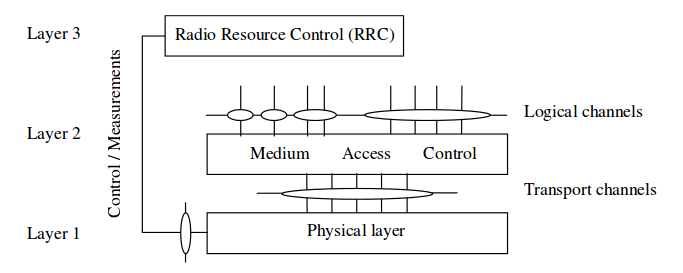
\includegraphics[width=3.5in]{figures3/protocolStack}
	\caption{E-UTRA radio interface protocol architecture.}
	\label{figs:stack}
\end{figure}
For both UL and DL, the physical transmission are divided into 

%TODO: Consider re-ordering
\subsection{LTE-A Physical Layer Protocol}
\label{lte-phy}
Description of both OFDMA and SC-FDMA, primarily researched/referenced from 3GPP TR 36.201 \cite{tr36201}. Consider including figures of both UL/DL framing, showing, from the point of view of Wi-Fi, that interference will/would span many WiFi transmission attempts (increased BO time due to no free channel time to decrement BO counter, resulting in significant frame delay, but not necessarily drops, but retransmission from the higher layers will likely cause drops from the queue .. ..  )  link adaptation? MIMO? not sure if this has any bearing on the issue at hand, but should probably be included for completeness
%TODO:Make figure
\begin{figure}[!ht] 
	\centering
	\subfloat[OFMDA used in downlink.]{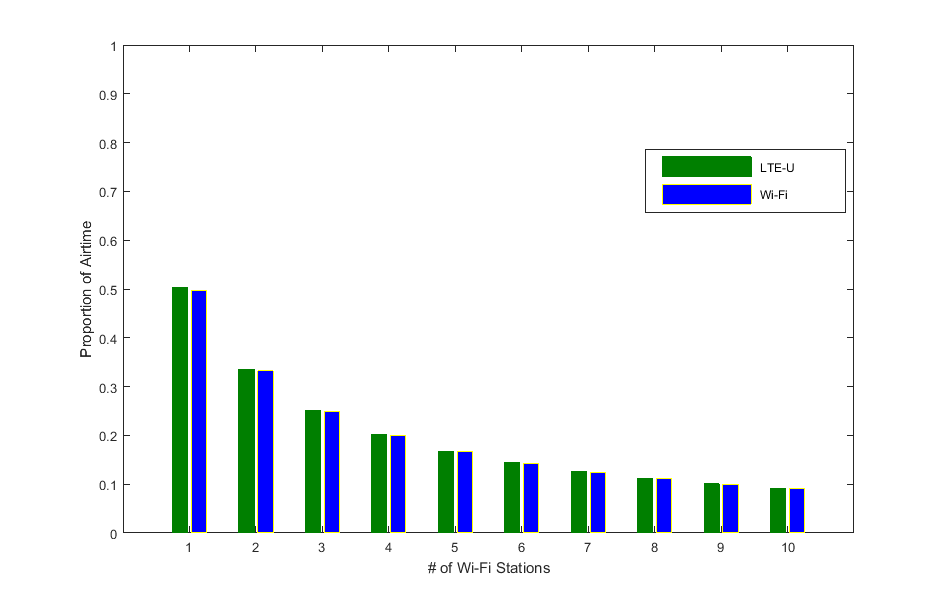
\includegraphics[width=2in]{figures/withadapt}%
		\label{ofdma}}
	\hfil
	\subfloat[SC-FDMA used in uplink.]{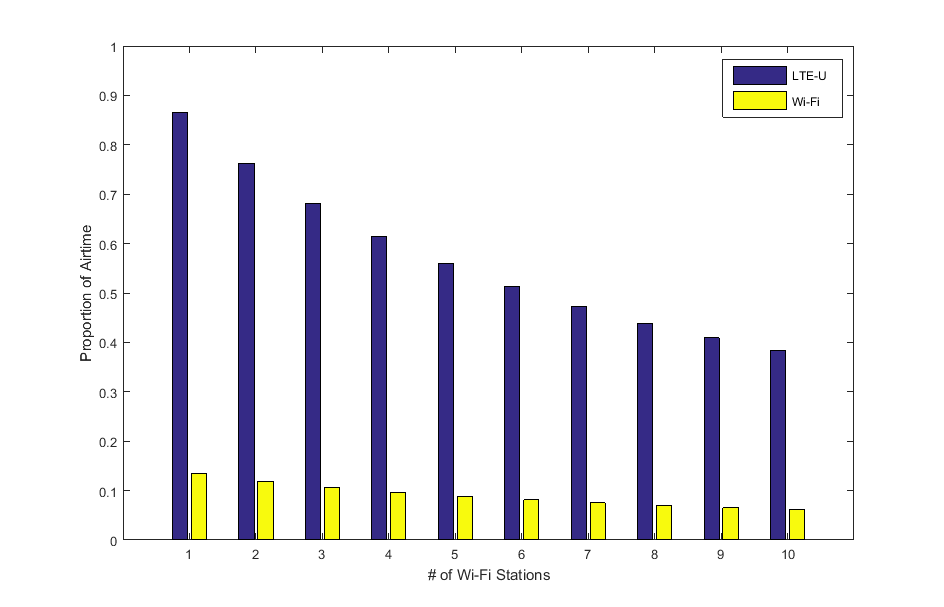
\includegraphics[width=2in]{figures/withoutadapt}%
		\label{sc-fdma}}
	\caption{PLACEHOLDER: Multiple access strategies used in LTE for uplink and downlink.}
	\label{fig:ofdma_sc-fdma_comp}
\end{figure}


\subsection{LTE-A Medium Access Protocol}
\label{lte-mac}
Description of (high-level) MAC sub-layer protocol activities and results, reference 3GPP TR 36.321 \cite{tr36321}
%Consider that the MAC layer is really not that important as some coexistence mechanism for the unlicensed channel will obviously need to be in place that will work in parallel to the MAC layer for controlling access to the licensed spectrum.


%TODO:Make figure
\begin{figure}[!ht]
	\centering
	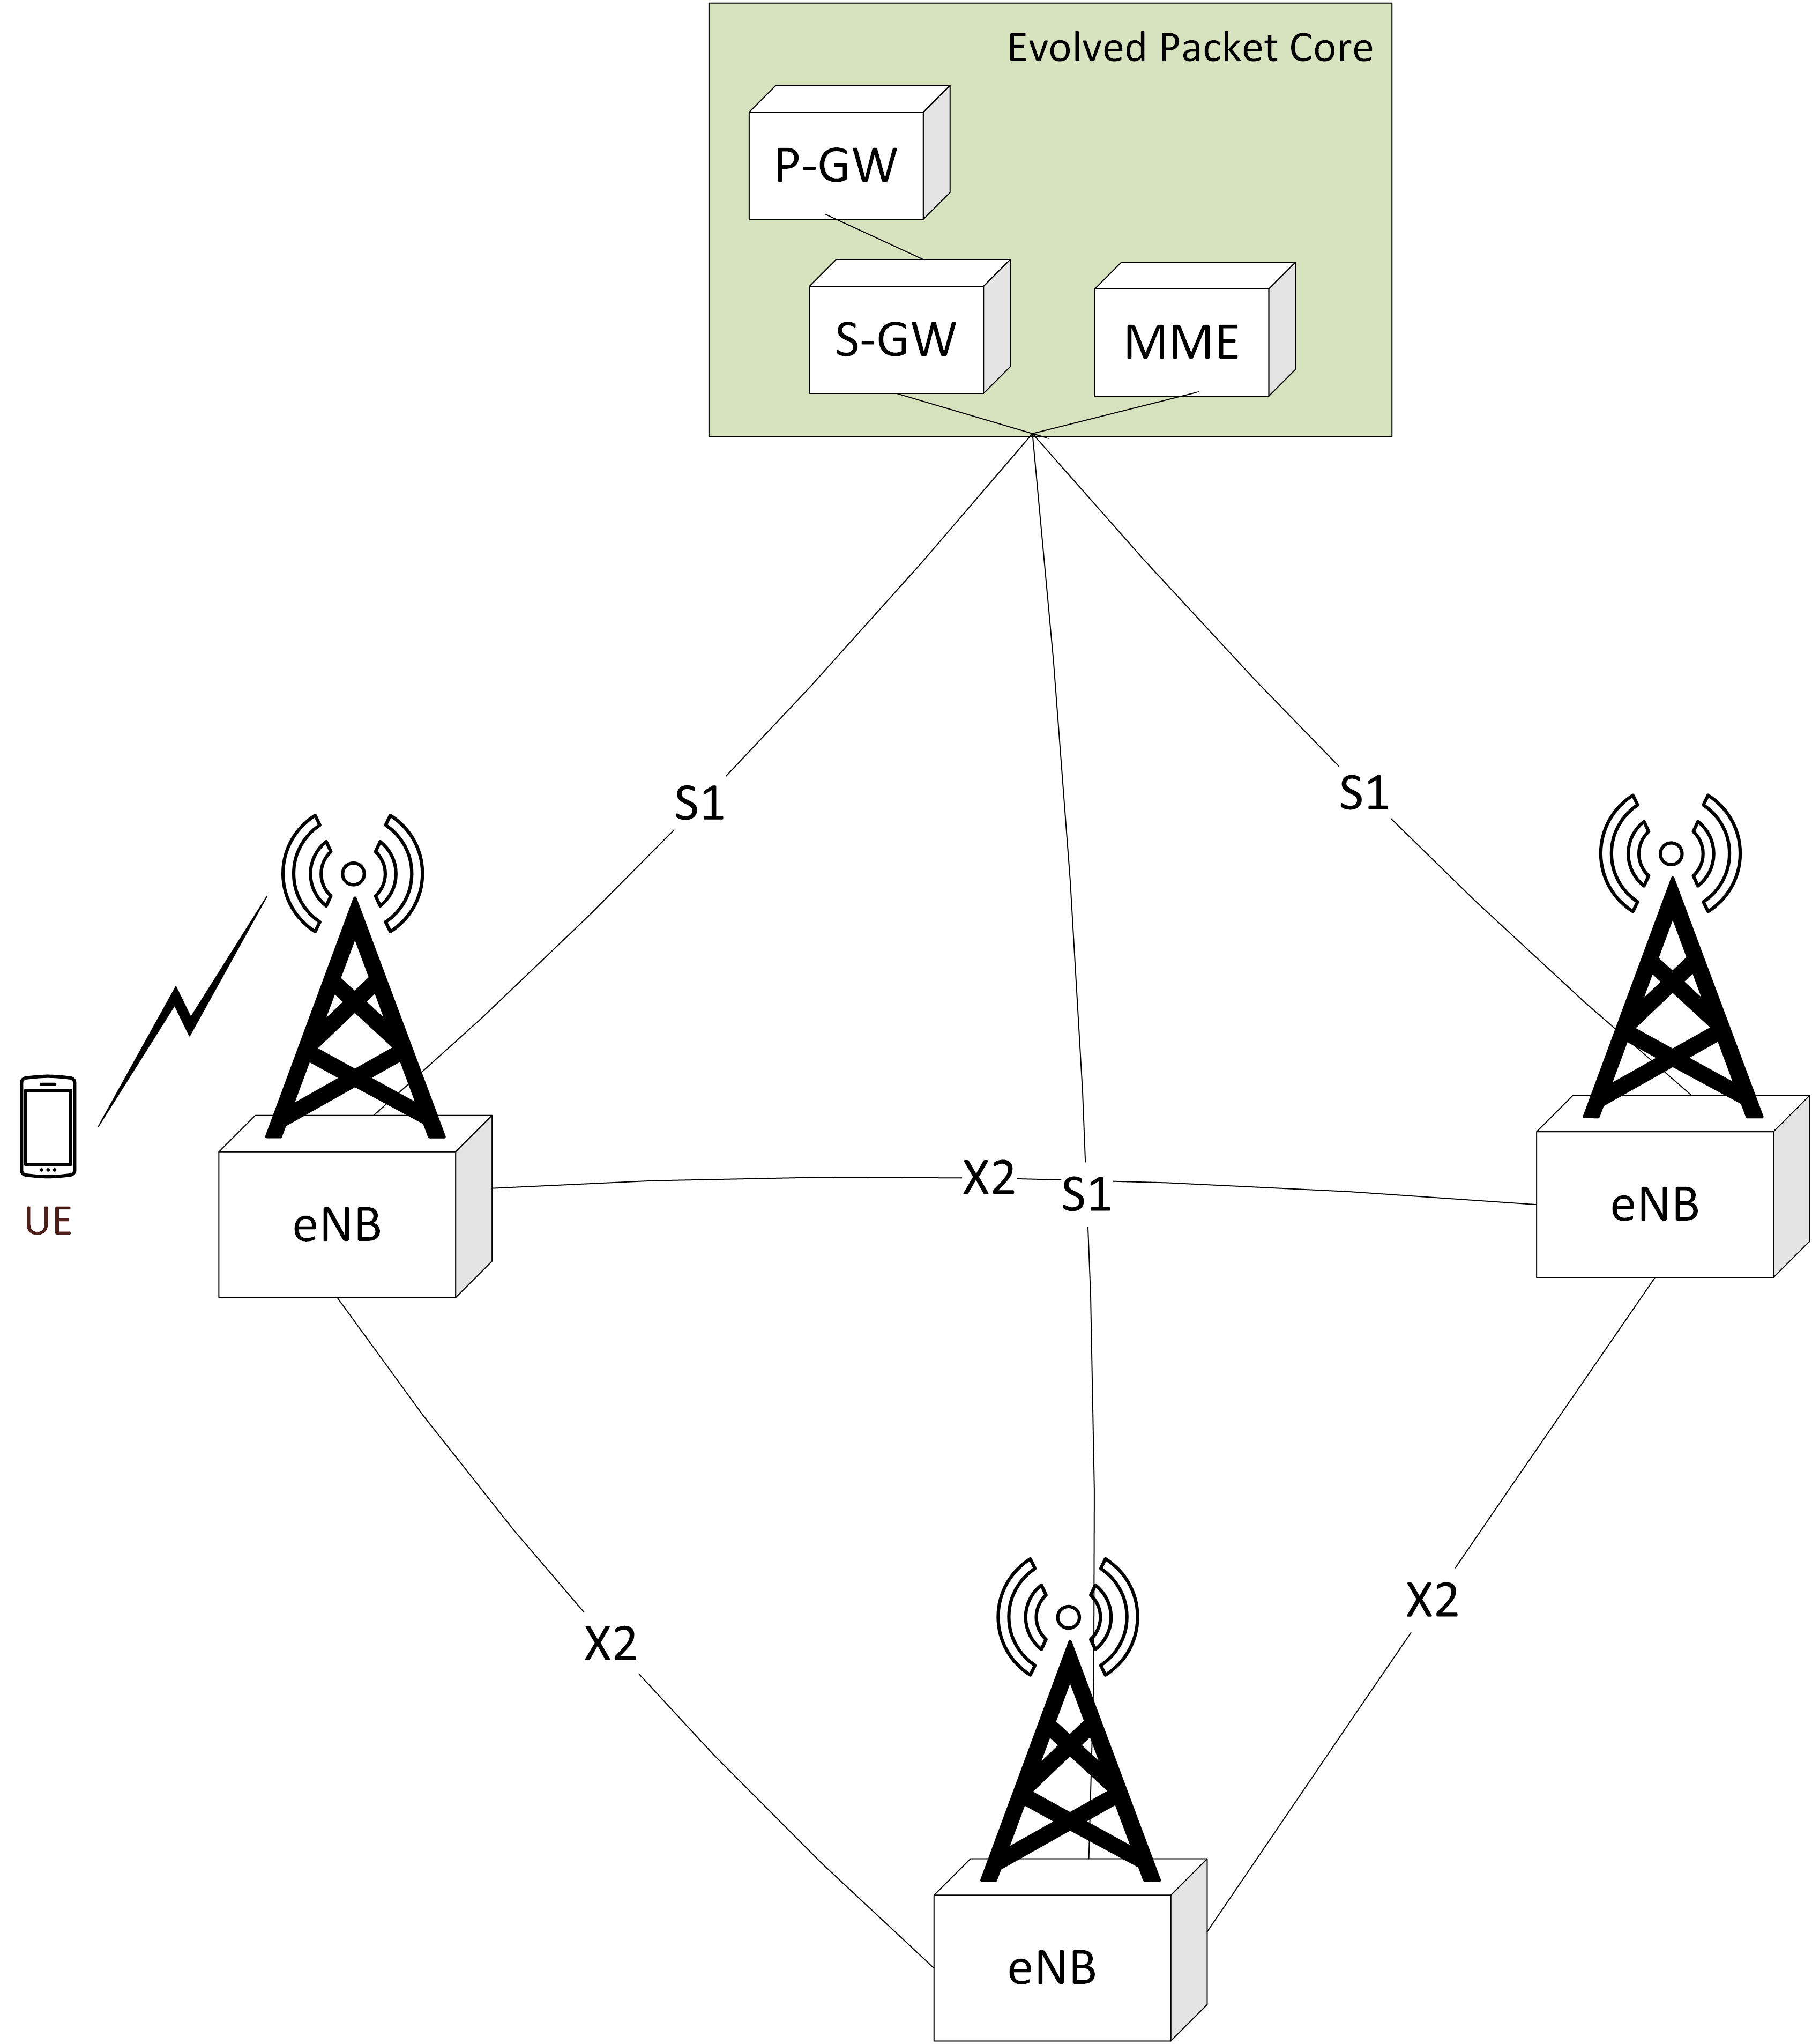
\includegraphics[width=2.5in]{figures3/lteAnet}
	\caption{PLACEHOLDER: LTE MAC sublayer detail.}
	\label{figs:LTE-MAC-protocol}
\end{figure}



%Consider section change to sources of coexistence issues
\section {Changes Expected for Future Releases}
\label{fut-chnge}
Brief outline of major work items which are expected to be included in releases 14/15 that could conceivably have any impact on LAA-LTE/WiFi coexistence, or are just really interesting features 
Possibly another table/chart

per 3GPP work plan available from their site (grab the citation at some later point) as well as the summary pages they have put together (see links saved in book refs folders)
%%%%%%%%%%%%%%%%%%%%%%%% referenc.tex %%%%%%%%%%%%%%%%%%%%%%%%%%%%%%
% sample references
% %
% Use this file as a template for your own input.
%
%%%%%%%%%%%%%%%%%%%%%%%% Springer-Verlag %%%%%%%%%%%%%%%%%%%%%%%%%%

\begin{thebibliography}{99.}%
	\bibitem{tr36913}{3GPP}, ``Requirements for further advancements for Evolved Universal Terrestrial Radio Access (E-UTRA) (LTE-Advanced),'' \emph{{3GPP TR 36.913 version 13.0.0 Release 10}}, 2011.
	\bibitem{lte-3gpp} 3GPP, ``{LTE},'' Whitepaper, ND. Accessed: June 21, 2016 [Online]. Available: \url{{www.3gpp.org/technologies/keywords-acronyms/98-lte}}
	\bibitem{itu-advanced}{ITU}, ``Requirements related to technical performance for IMT-Advanced radio interface(s),'' \emph{Rep. ITU-R M.2134}, 2008. 
	\bibitem{tr25.913}{3GPP}, ``Requirements for Evolved UTRA (E-UTRA) and Evolved UTRAN (E-UTRAN),'' \emph{{3GPP TR 25.913 version 8.0.0 Release 8}}, 2009.
	\bibitem{tr36321}{3GPP}, ``Evolved Universal Terrestrial Radio Access (E-UTRA); Medium Access Control (MAC) protocol specification,'' \emph{{3GPP TR 36.321 version 13.1.0 Release 13}}, 2016.
	\bibitem{tr36201}{3GPP}, ``Evolved Universal Terrestrial Radio Access (E-UTRA); LTE physical layer; General description,'' \emph{{3GPP TR 36.201 version 13.1.0 Release 13}}, 2016.	
\end{thebibliography}